\documentclass{report}
\usepackage{setspace} % Setting line spacing
\usepackage{ulem} % Underline
\usepackage{caption} % Captioning figures
\usepackage{subcaption} % Subfigures
\usepackage{geometry} % Page layout
\usepackage{multicol} % Columned pages
\usepackage{array,etoolbox}
\usepackage{fancyhdr}
\usepackage{enumitem}
\usepackage[toc,page]{appendix}
\setlist{noitemsep}

% Page layout (margins, size, line spacing)
\geometry{letterpaper, left=1in, right=1in, bottom=1in, top=1in}
\setstretch{1.15}

% Headers
\pagestyle{fancy}
\lhead{PeaPod - Solution Overview}
\rhead{UTAG}

% Metric counter, referencing commands
\newcounter{metricnumber}
\setcounter{metricnumber}{1}
\newcommand{\metricrow}{M\arabic{metricnumber}}
\newcommand{\mlabel}[1]{\addtocounter{metricnumber}{-1}\refstepcounter{metricnumber}\label{#1}\addtocounter{metricnumber}{1}}
\newcommand{\mref}[1]{M\ref{#1}}

\begin{document}

\begin{titlepage}
    \begin{center}
        \vspace*{1.2cm}

        \textbf{\large{PeaPod - Solution Overview}}

        \vspace{0.5cm}

        Outlining a Proposal to the PeaPod Requirements

        \vfill

        Jayden Lefebvre - Lead Engineer\\\small{jayden.lefebvre@mail.utoronto.ca}\\
        \vspace{1cm}
        Nathan Chareunsouk, Navin Vanderwert, Jonas Marshall - Design Engineers

        \vspace{2.5cm}

        Revision 0.4\\
        University of Toronto Agritech\\
        July 7th, 2021

    \end{center}
\end{titlepage}

\thispagestyle{plain}

\tableofcontents
\newpage

\section{Introduction}
\label{sec:intro}

\subsection{Purpose \& Design Process}
\label{sec:purpose}

The purpose of this document is to outline a design proposed to meet the PeaPod Requirements.

It accomplishes this via the following process:

\begin{figure}[h]
    \centering
    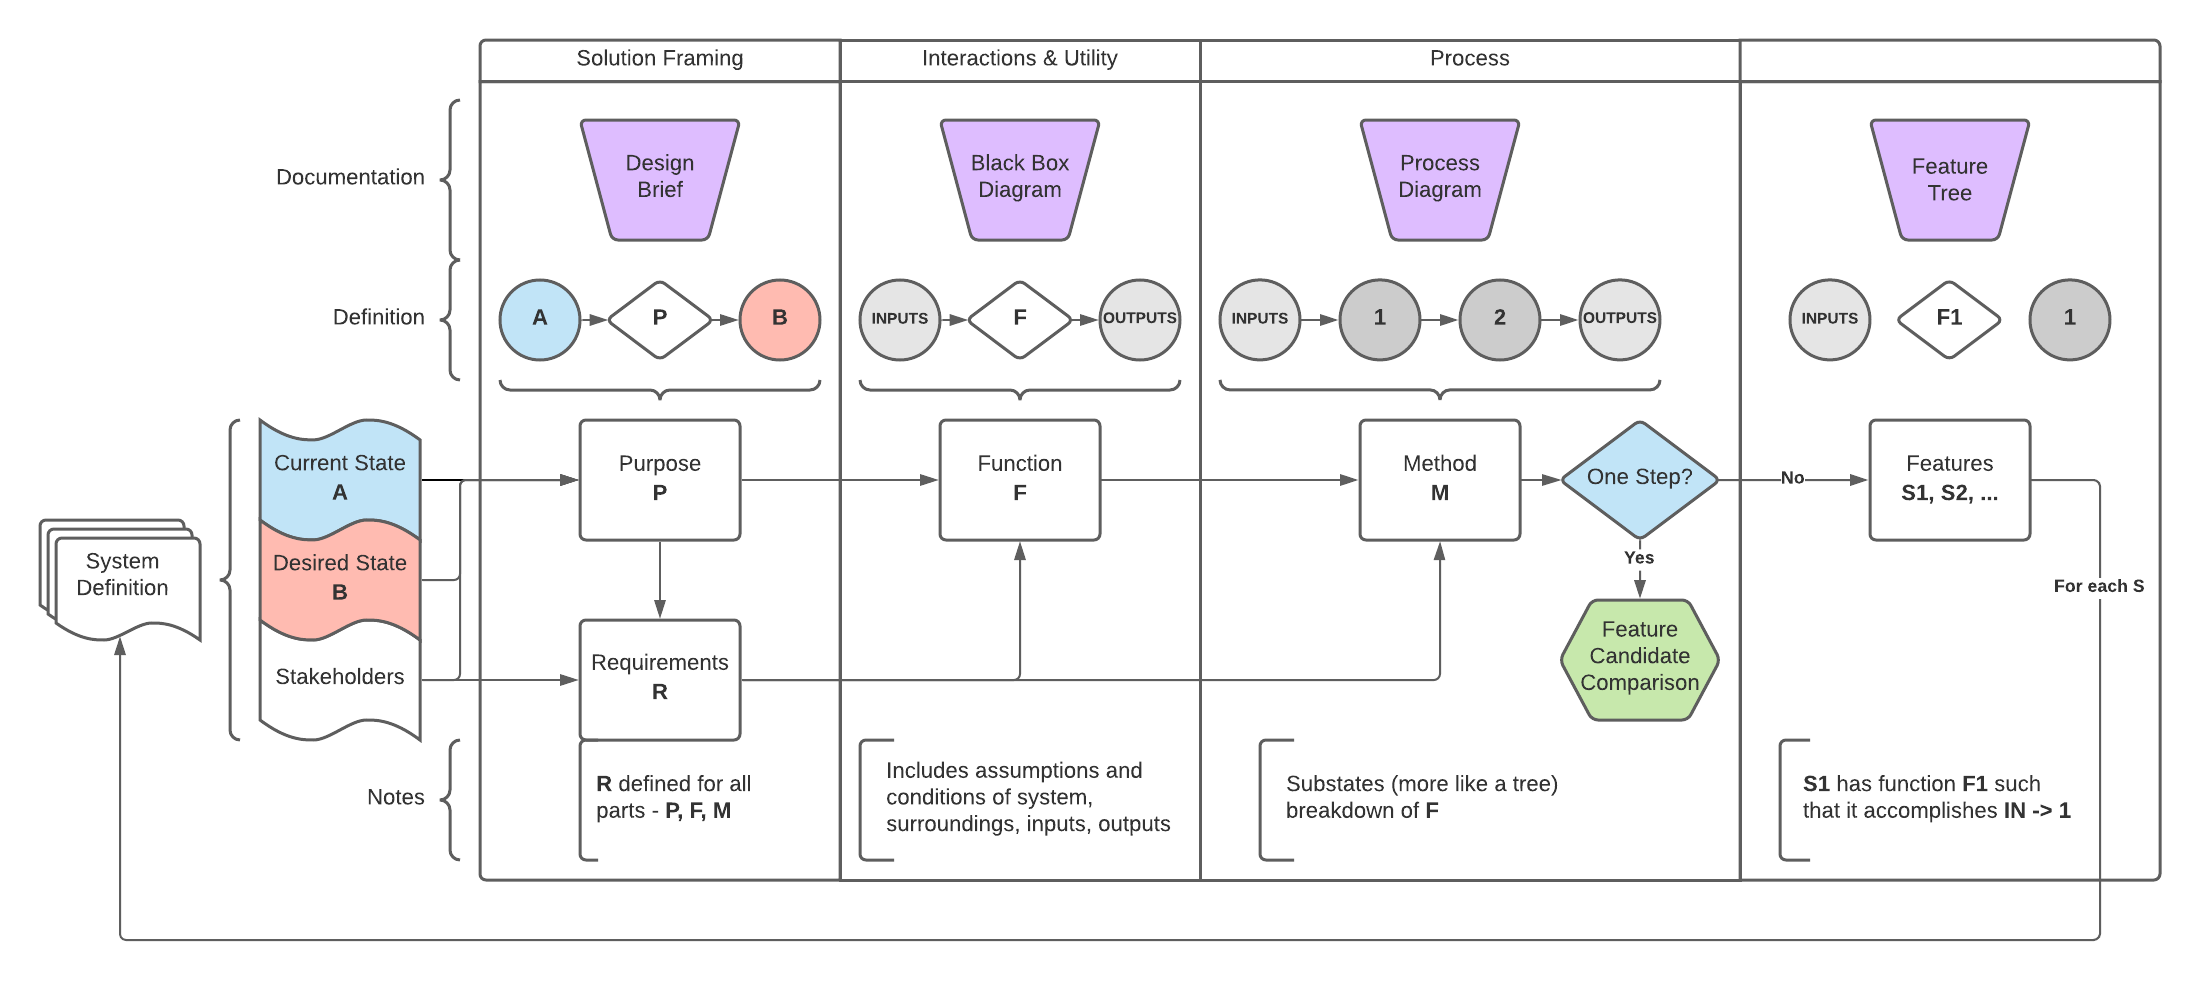
\includegraphics[width=17cm]{images/designprocess.png}
    \hfill
    \caption{Engineering design process.}
\end{figure}

\newpage

\section{Design}

\textbf{Purpose}: The purpose of the design is derived from the opportunity statement:

PeaPod is "an \uline{automated} and \uline{isolated} \uline{aeroponic} crop growth system, able to generate any \uline{growth environment} from a combination of independent \uline{environment parameters}, with both environment and crop growth \uline{data collection} for \uline{optimization}".

The primary function of the overall design are derived from both the overall purpose as well as the system inputs and outputs as defined by the DSFC Applicant Guide \cite{applicantguide}.

\textbf{Function}:

\begin{figure}[h]
    \centering
    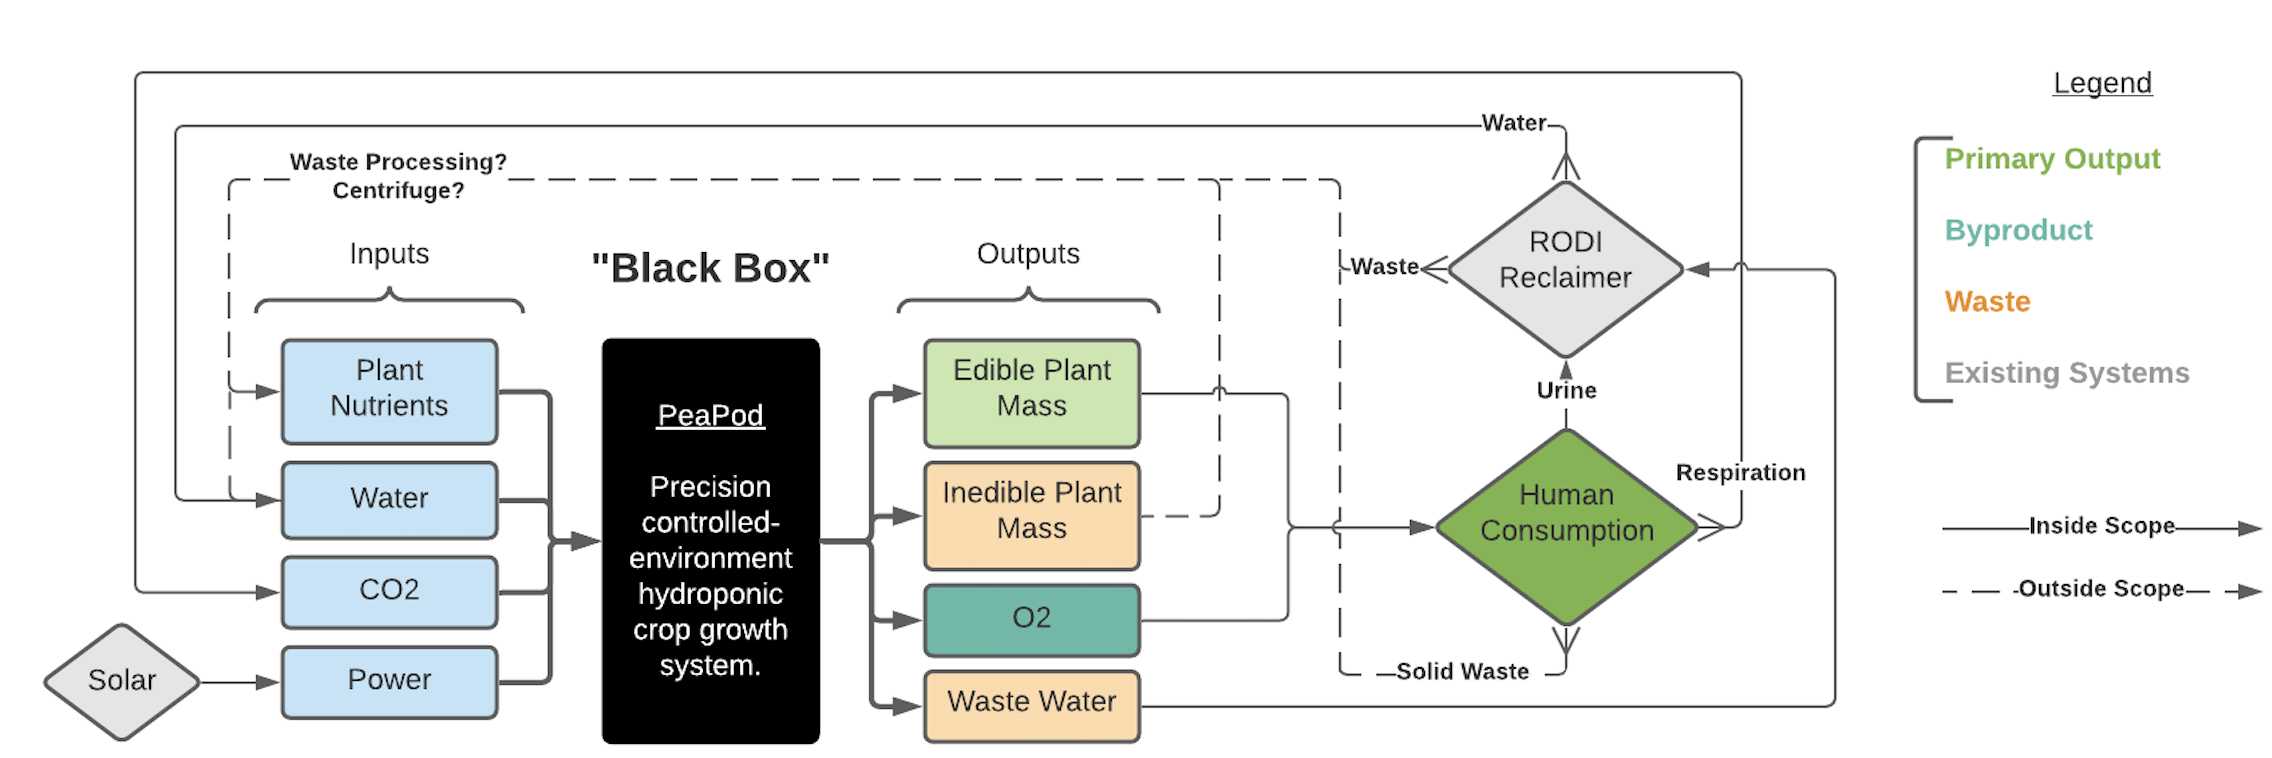
\includegraphics[width=15cm]{images/blackbox.png}
    \hfill
    \caption{"Black box" function diagram of PeaPod.}
\end{figure}

\textbf{Method \& Features}: 

\begin{figure}[h]
    \centering
    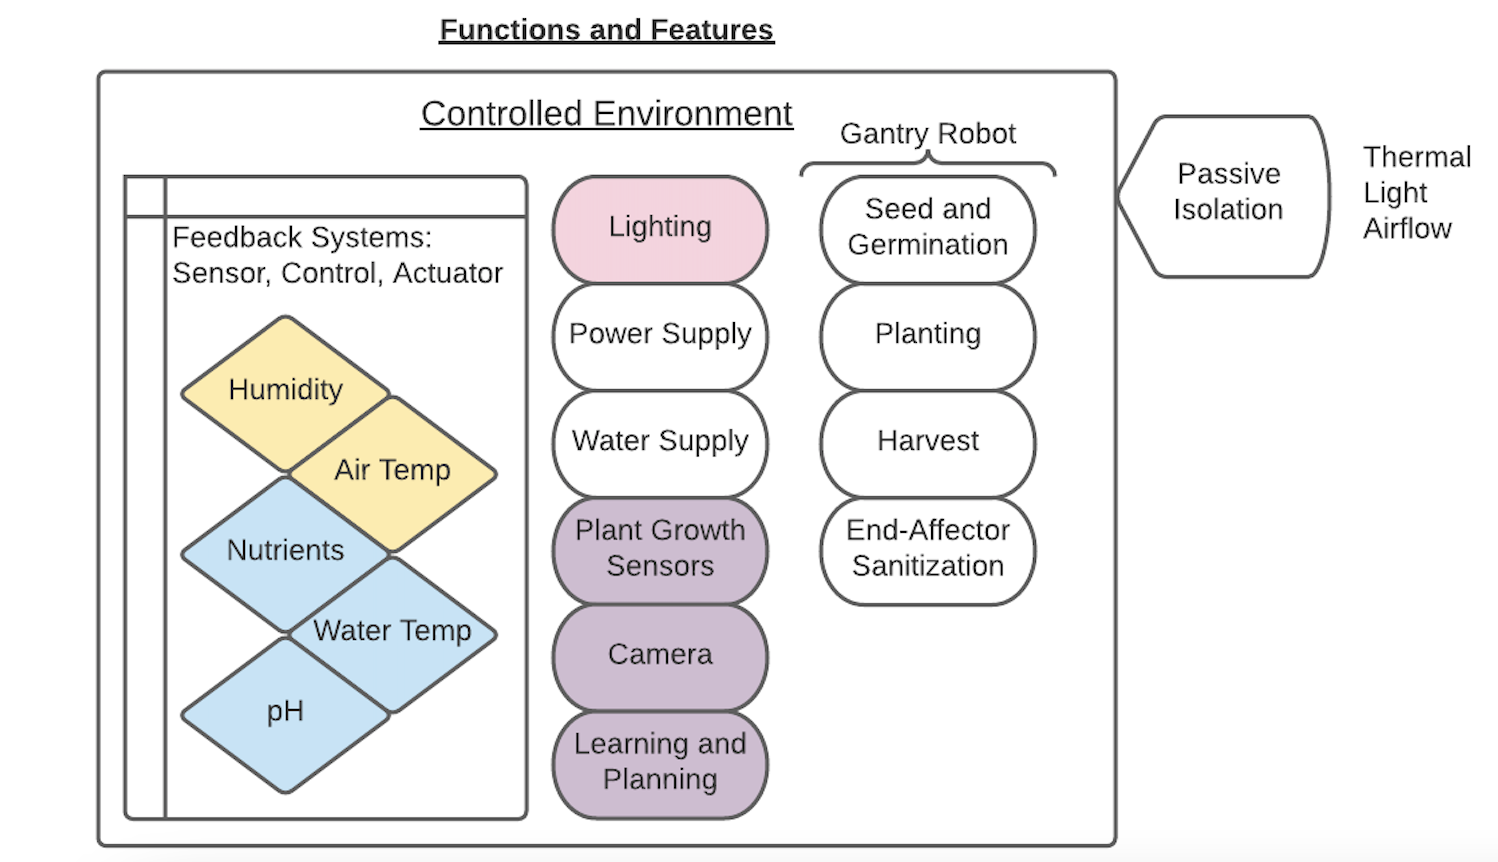
\includegraphics[width=12cm]{images/features.png}
    \hfill
    \caption{Features and feature types of PeaPod.}
\end{figure}

\newpage

\subsection{Automation}
\label{sec:automation}

\textbf{Purpose}: Performing growth-, maintenance-, and data-related tasks autonomously on the basis of both schedule and necessity to reduce crew maintenance time. Maintains the homogeneity of the internal environment.

\textbf{Function}:
\begin{itemize}
    \item \textbf{Inputs}: Environment sensor reading signals, program
    \item \textbf{Outputs}: Actuator control signals, crew messaging
\end{itemize}

\textbf{Method}:
\begin{enumerate}
    \item User inputs program:
    \begin{itemize}
        \item Action-at-timestamp, e.g. lights on at 08:00;
        \item Control target with start/end, e.g. hold air temperature at 22°C from 11:00 to 18:00;
    \end{itemize}
    \item Notification on maintenance requirement (i.e. non-automated input/output management, refills, repairs, etc.);
    \item "Sense, Plan, Act" robotics/control model:
    \begin{enumerate}
        \item \textit{Senses} current conditions;
        \item \textit{Plans} a path to desired condition;
        \item \textit{Acts} to change current condition to desired condition;
    \end{enumerate}
\end{enumerate}

\textbf{Features}:
\begin{itemize}
    \item Central \textbf{computer system} with internal clock and network connection;
    \item Environment sensors (\textit{Sense}) for each \textbf{environmental control} (\ref{sec:environment});
    \item \textbf{Program} of time-series and/or control target instructions (\textit{Plan});
    \item Actuators (\textit{Act}) for each \textbf{environmental control} (\ref{sec:environment});
\end{itemize}

\textbf{Justification}: 
\begin{itemize}
    \item \textbf{Purpose}: Increased accuracy/precision over human interference, minimize human hours spent. Enables control over all parameters simultaneously.
    \item \textbf{Method}: Data structure matches $\vec E$ from the optimization routine (see Section \ref{sec:optimization}). Control loop-style topology is common is well suited for controlled-environment agriculture.
\end{itemize}

% \subsubsection{Computer System}
% \label{sec:computer}

% \textbf{Purpose}: Primary operating infrastructure. Automation, data transmission, remote control.

% \textbf{Function}:
% \begin{itemize}
%     \item \textbf{Inputs}: Power, network connection, input signals
%     \item \textbf{Outputs}: Output signals
% \end{itemize}

% \textbf{Method}:

% \textbf{Features}:

% \textbf{Justification}:
% \begin{itemize}
%     \item \textbf{Purpose}:
%     \item \textbf{Method}:
% \end{itemize}

% \subsubsection{Program}
% \label{sec:program}

% \textbf{Purpose}: Set of environment parameter instructions for the automation system.

% \textbf{Function}:
% \begin{itemize}
%     \item \textbf{Inputs}:
%     \item \textbf{Outputs}:
% \end{itemize}

% \textbf{Method}:

% \textbf{Features}:

% \textbf{Justification}:
% \begin{itemize}
%     \item \textbf{Purpose}:
%     \item \textbf{Method}:
% \end{itemize}

\newpage

\subsection{Housing}
\label{sec:housing}

\textbf{Purpose \& Function}: \textit{Isolates} and \textit{Insulates} growth environment from exterior environment (heat, light, humidity). Provides structural integrity and mounting points for other subsystems (\textit{Frame}).

\textbf{Method}:
\begin{itemize}
    \item Insulation (\textit{keep in}):
    \begin{itemize}
        \item Heat - Insulative/reflective internal shell
        \item Light - Reflective internal shell
        \item Moisture - "Sealed" shell
    \end{itemize}
    \item Isolation (\textit{keep out}):
    \begin{itemize}
        \item Heat - Insulative shell
        \item Light - Opaque shell
        \item Moisture - "Sealed" shell
    \end{itemize}
    \item $\therefore$ Frame skeleton w/ solid, internally-reflective, "sealed" panels;
    \item Standard subframes for mounting entire subsystems modularly;
\end{itemize}

\textbf{Features}:
\begin{itemize}
    \item Aluminum extrusion skeleton w/ standard mounting channels;
    \item Foam insulation panels w/ mylar internal coating slide into exoskeleton channels;
    \item Trays - base subframe unit, adaptable; mounted to vertical internal channels for vertical repositioning; all connections are \textit{quick-disconnect} (i.e. quick-connect tubing for grow tray, push connectors for lighting):
    \begin{itemize}
        \item Grow trays - Support plants (via grow cups), aeroponic nozzles (See \ref{sec:aeroponics}, and misting container.
        \item Lighting trays - Support LED boards, driver board (See \ref{sec:lighting}).
    \end{itemize}
\end{itemize}

\textbf{Justification}: 
\begin{itemize}
    \item \textbf{Function}: Insulation increases thermal and light efficiency. Isolation increases safety against cross-contamination, pathogens, harmful substances.
    \item \textbf{Method}: Solid frame-and-panel construction is efficient for packing away, and is honestly just simple. Adaptable tray subframes make future feature development easier, and allows to modularly swap subsystems.
    \item \textbf{Features}: Aluminum extrusion is commonly used for frames. Allows strong, repositionable mounting via channels. Foam insulation is highly insulative and opaque, and mylar ensures internal light reflection. Sliding directly into extrusion channels boosts "seal".
\end{itemize}

\newpage

\subsection{Aeroponics}
\label{sec:aeroponics}

\textbf{Purpose}: Delivers \textit{nutrients} and \textit{pH}-balanced, \textit{temperature}-controlled \textit{water} to the plants via a \textit{fine mist} (~50 micron mean droplet diameter).

\textbf{Function}:
\begin{itemize}
    \item \textbf{Inputs}: Filtered/RO water under positive pressure, pH up \& down solutions, concentrated nutrient solutions, pump control (on/off relay to pump power), nozzle control (on/off relay to solenoid)
    \item \textbf{Outputs}: Mist
\end{itemize}

Utilizing a diaphram pump and pressure accumulator tank, filtered water with correct ph and nutrient concentration is pressurized to 80 psi before being atomized by the nozzle and subsequently abosorbed by the roots.

\textbf{Method}:
\begin{itemize} 
    \item Water is sourced from an external RO system with positive pressure;
    \item Water is pressurized to constant 80psi;
    \item Water is heated or cooled to a given temp (\ref{sec:automation}); % TODO: Add water temp to environment control?
    \item Nutrient and pH-adjustment solutions are mixed in-line at an adjustable ratio (\ref{sec:automation}); \footnote{I.e. add X mL of nutrient solution Y per mL water to achieve Z ppm, or add A mL of pH down solution per mL water to achieve a pH of B.}
    \item Flow to nozzle is controlled (on/off) (\ref{sec:automation}
    );
    \item Nozzle turns pressurized water into mist;
\end{itemize}

\textbf{Features} (in order of plumbing; source $\to$ nozzle):
\begin{itemize}
    \item \textit{Water Source}: Input for filtered, reverse-osmosis water.
    \item \textit{Diaphragm Pump}: Self-priming, auto-shutoff at 80psi. Power is controlled by external relay signal (\ref{sec:automation}).
    \item \textit{Inline Water Heater/Cooler}: Thermoelectric heater/cooler
    \item \textit{Accumulator Tank}: Uses an air bladder to create and stabilize pressure.
    \item \textit{Pressure Sensor} reports to computer (\ref{sec:automation}). Allows for shutoff of pump in case of emergency.
    \item \textit{Adjustable-rate Siphon Injection Manifold}: A set of venturi-based siphon injectors for flow-ratio siphoning of solutions (onen siphon per solution). See \ref{sec:manifold}.
    \item \textit{Solenoid Valve} - Enables on-demand (\ref{sec:automation}) misting.
    \item \textit{Grow Tray Quick-Disconnect}: Connectors between aeroponics supply and nozzles that allow for quick disconnection with auto-shutoff so the trays may be removed.
    \item \textit{Nozzle}: Mounted to grow tray, pointed at plant roots. 80psi water through a 0.4$\to$0.6mm orifice produces 5$\to$50 micron water droplets. %TODO: Source??
\end{itemize}

\newpage

\textbf{Justification}: 
\begin{itemize}
    \item \textbf{Purpose}: A high pressure aeroponics system eliminates water parameter feedback, and is 98\% more water efficient than traditional farming.
    \item \textbf{Function}: RO water has no dissolved nutrients and a neutral pH of 7.0. This enables easier and more reliable calculations. In addition, it has no particulate or minerals, minimizing the chances of nozzle clog.
    \item \textbf{Method}: System is medium-free, eliminating risk of pathogens developing within root zone. Using a nozzle ensures the nutrient solution is evenly distributed. 5-50 micron mean droplet size is optimal for plant growth. %TODO: Source?? also more detail here
\end{itemize}

\subsubsection{Solution Injection Manifold}
\label{sec:manifold}

\textbf{Purpose}: A manifold of venturi-based \textit{siphons} for in-line, \textit{adjustable flow-ratio} injection and mixing of nutrient and pH-adjustment solutions.

\textbf{Function}:
\begin{itemize}
    \item \textbf{Inputs}: Pressurized RO water, per-solution flow-ratio control signal (calculated from desired per-nutrient concentrations; \ref{sec:automation}), pH flow-ratio control signal (calculated from desired pH; \ref{sec:automation})
    \item \textbf{Outputs}: Pressurized mixed solution with set pH and nutrient concentrations
\end{itemize}

\textbf{Method}:
\begin{enumerate}
    \item Manifold splits off into branches (one per solution)
    \item Each solution branch:
    \begin{itemize}
        \item A venturi siphon for fixed flow-ratio injection;
        \item An adjustable-flow valve controlling solution flow rate;
    \end{itemize}
    \item Manifold recombines
\end{enumerate}

\textbf{Features}:
\begin{itemize}
    \item \textit{Siphon Injectors}
    \item \textit{Needle Valves}: Completely adjustable flow control
    \item \textit{One-way Valves}: Prevents backflow through siphon inlet
\end{itemize}

% TODO: Justification?

\newpage

\subsection{Environment Control}
\label{sec:environment}

\textbf{Purpose}: Generating the internal plant growth environment, with control over all relevant environment parameters:
\textbf{Function}:
\begin{itemize}
    \item \textbf{Inputs}: Power, water, environment control parameters (as signals)
    \item \textbf{Outputs}: Controlled environment (optimal for plant growth)
\end{itemize}

\textbf{Method} (informed by \ref{sec:automation}):
\begin{itemize}
    \item Control System Parameters:
    \begin{itemize}
        \item Leaf zone air temperature;
        \item Leaf zone humidity;
        \item Root zone/aeroponics spray temperature;
    \end{itemize}
    \item Set Parameters:
    \begin{itemize}
        \item Lighting spectrum and intensity;
        \item Aeroponics delivery/"flow" rate;
        \item Aeroponics solution per-nutrient concentrations;
        \item Aeroponics solution pH;
    \end{itemize}
\end{itemize}

\textbf{Features}:
\begin{itemize}
    \item \textit{Air Heater, Cooler} (\ref{sec:airtemp})
    \item \textit{Air Humidifier} (\ref{sec:airhum}), \textit{Dehumidifier} (\ref{sec:dehum})
    \item \textit{Aeroponics System} (\ref{sec:aeroponics}), with:
    \begin{itemize}
        \item \textit{Solution Heater, Cooler} (\ref{sec:watertemp})
        \item \textit{Solution Dosing} (\ref{sec:nutrients}, \ref{sec:ph})
    \end{itemize}
    \item \textit{Lighting} (\ref{sec:lighting})
\end{itemize}

\subsubsection{Air Temperature}
\label{sec:airtemp}

\textbf{Purpose}: Maintaining desired air temperature within the enclosure.

\textbf{Function}:
\begin{itemize}
    \item \textbf{Inputs}: Power, air temperature control signal (\ref{sec:automation})
    \item \textbf{Outputs}: Heating/cooling, air circulation, air temperature signal (\ref{sec:automation})
\end{itemize}

\textbf{Method}:
\begin{itemize}
    \item Air is circulated and temperature is measured;
    \item Temperature is used to inform control signal;
    \item Heat is pumped into or out of the box (direction and magnitude depending on the control signal) and radiated;
\end{itemize}

\textbf{Features}:
\begin{itemize}
    \item \textit{Temperature Sensors}: Located throughout the growth environment to measure air temperature. Informs a PID control loop (\ref{sec:automation});
    \item \textit{Peltier Devices}: Pumps heat from one side of a tile to the other via the thermoelectric effect. Direction and magnitude of heat transferred depends on control signal polarity (\textit{H-bridge}) and voltage (respectively).
    \item \textit{Heat Sinks}: Connected to peltier devices. Exchanges heat between air and peltier devices.
    \item \textit{Fans}: Located on heat sinks and in growth environment to circulate air for better heat dispersal and even temperature distribution.
\end{itemize}

\textbf{Justification}: 
\begin{itemize}
    \item \textbf{Function}: Air management ensures an even temperature throughout the entire growth environment. Thermal exchange effectively pumps heat into or out of the growth envrionment.
    \item \textbf{Features}: Peltier devices have better space and energy efficiency, less complexity (no liquids, pressurized fluids, etc.), and can provide precise temperature control at low voltages through automation via methods such as PID. They can also operate as both heaters and coolers, and can be easily controlled electrically.
\end{itemize}

\newpage

\subsubsection{Air Humidification}
\label{sec:airhum}

\textbf{Purpose}: Increasing air humidity on command.

\textbf{Function}:
\begin{itemize}
    \item \textbf{Inputs}: Power, humidification on/off control signal (\ref{sec:automation}), RO water;
    \item \textbf{Outputs}: Water vapour;
\end{itemize}

\textbf{Method}:
\begin{enumerate}
    \item Power and control signal activate a nebulizer driver;
    \item Water is delivered to the nebulizer and nebulized;
\end{enumerate}

\textbf{Features}:
\begin{itemize}
    \item \textit{Driver Circuit}: Fixed-frequency (113kHz) 555 timer circuit driving an amplifier/LC circuit generates a 25V AC signal. %TODO: why 113kHz?
    \item \textit{Mesh Piezo Disc}: Driven by the circuit, generates a vapour when water is passed over it.
\end{itemize}

\textbf{Justification}:
\begin{itemize}
    \item \textbf{Function}: RO water contains no minerals/particulate, and as such prevents the common problem of piezo/mesh calcification.
    \item \textbf{Method \& Features}: The nebulizer approach is easily electrically controllable and produces a consistent fine vapour. 
\end{itemize}

\subsubsection{Air Dehumidification}
\label{sec:dehum}

\textbf{Purpose}: \textit{Removes moisture} from the growth environment on demand. Used in conjunction with humidity sensor and humidification system to maintain a desired humidity.

\textbf{Method}:
\begin{itemize}
    \item Circulation (\textit{moving air through system}):
    \begin{itemize}
        \item Chamber - Where air is dehumidified. Only one in, and one out.
        \item Fan - Blows air into the growth environment from chamber, subsequently draws air through humidification system.
        \item Filter - HEPA filter is located at inlet of chamber. Eliminates risk of any airborn pathogens being transferred onto silica beads.
        \item Shutters - Isolates dehumidification chamber when not in use. One located at chamber inlet, and one located at chamber outlet. 
    \end{itemize}
    \item Dehumidification (\textit{remove moisture from air}):
    \begin{itemize}
        \item Cartridge - Holds silica beads. Allows beads to be removed quickly and easily.
        \item Silica Beads - Absorbs moisture from air passed around it.
    \end{itemize}
    \item Rejuvenation (\textit{remove moisture from silica}):
    \begin{itemize}
        \item Evaporator - Warms cartridge to evaporate moisture collected by silica beads.
    \end{itemize}
\end{itemize}

\textbf{Features}:
\begin{itemize}
    \item Silica gel beads provide very efficient dehumidification.
    \item Silica beads are non-toxic.
    \item Silica beads are completely passive and require no active electricity (aside from shutters and fans).
    \item Silica beads change color to indicate saturation.
    \item Silica beads can be easily reused by drying them out. Moisture can be captured during the drying process and be recycled.
\end{itemize}

\textbf{Justification}: 
\begin{itemize}
    \item \textbf{Function}: Silica beads are completely passive and provide very efficient dehumidification.
    \item \textbf{Method}: Cartridges make replacing the silica beads very quick and easy. 
    \item \textbf{Features}: Silica gel is non-toxic and non-organic. Silica beads can be sourced easily and are not too expensive. Silica beads change color to indicate saturation, making it easy to tell when they need to be rejuvenated.
\end{itemize}

\newpage



\subsubsection{Solution Temperature}
\label{sec:watertemp}

\textbf{What}: Maintaining desired water temperature within the water store.

\textbf{How}: Same as \ref{sec:airtemp}; on a water block.

\textbf{Why}: Same as \ref{sec:airtemp}.

\subsubsection{Solution Nutrients}
\label{sec:nutrients}

\textbf{Function}: Formulates the correct concentration of nutrient solution by \textit{precisely injecting} the correct amounts of nutrient solution into the water stream.

\textbf{Method}:
\begin{itemize}
    \item Water Supply (\textit{water into system}):
    \begin{itemize}
        \item RO System - External filtration system. 
        \item Unidirectional Valve - Located between RO system and venturi syphons to prevent backflow into RO system.
        \item Pump - Same pump as \ref{sec:aeroponics}. Draws water from RO system.
    \end{itemize}
    \item Injection (\textit{mixing solution into water stream}):
    \begin{itemize}
        \item Venturi Syphon - Located between unidirectional valve and pump. Creates a vacuum that draws nutrient solution into main water stream.
        \item Proportional Control Solenoid - Located at side inlet of venturi syphon. Enables controlling flow of nutrient solution into water stream.
        \item Unidirectional Valve - Located between proportional control solenoid and nutrient solution container. Prevents dilution of nutrient solution container.
        \item Nutrient Solution Container - Holds nutrient solutions.
    \end{itemize}
    \item Control (\textit{maintaining solution ratio}):
    \begin{itemize}
        \item Flow Sensor - Located at intlet of venturi syphon. Measures flow into venturi syphon.
        \item Solution Sensor - Located at outlet of venturi syphon. Measures solution concentration. Data is combined with flow sensor to control the porportional solenoid valve through automation.
    \end{itemize}
    \item $\therefore$ All appropriate fittings and tubing.
\end{itemize}

\textbf{Features}:
\begin{itemize}
    \item Venturi syphon is passive and relies on the main pump to draw solution into main stream.
    \item Proportional control solenoid is very precise and allows for precision control over solution ratio.
    \item System has minimal moving parts which increases reliability.
    \item Both venturi syphon and proportional control solenoid can be bought as off the shelf components.
\end{itemize}

\textbf{Justification}: 
\begin{itemize}
    \item \textbf{Function}: Water supply moves water into system. Injection formulates correct solution ratio. Control enables injection management through automation.
    \item \textbf{Method}: This system enables precise inline solution injection which eliminates need for a resevoir. Proportional control solenoid allows for very precise control of solution ratio. Venturi syphon is completely passive, completely eliminating the need for a solution pump. 
    \item \textbf{Features}: All parts are common and can be bought off the shelf. Venturi syphon is a proven reliable way to mix solution into a main stream. Is used in many applications from paint sprayers to fertilizer injectors.
\end{itemize}

\newpage


\subsubsection{Solution pH}
\label{sec:ph}

\textbf{Function}: Formulates the correct pH of the solution by \textit{precisely injecting} the correct amounts of pH up/down solutions into the water stream.

\textbf{Method}:
\begin{itemize}
    \item Water Supply (\textit{water into system}):
    \begin{itemize}
        \item RO System - External filtration system. 
        \item Unidirectional Valve - Located between RO system and venturi syphons to prevent backflow into RO system.
        \item Pump - Same pump as \ref{sec:aeroponics}. Draws water from RO system.
    \end{itemize}
    \item Injection (\textit{mixing solution into water stream}):
    \begin{itemize}
        \item Venturi Syphon - Located between unidirectional valve and pump. Creates a vacuum that draws nutrient solution into main water stream.
        \item Proportional Control Solenoids - Located at side inlet of venturi syphon. Enables controlling flow of pH up/down solutions into water stream. One for each solution.
        \item Unidirectional Valve - Located between proportional control solenoid and nutrient solution container. Prevents dilution of pH up/down solution containers.
        \item pH Solution Containers - Holds pH up/down solutions. One for each solution.
    \end{itemize}
    \item Control (\textit{maintaining solution ratio}):
    \begin{itemize}
        \item Flow Sensor - Located at intlet of venturi syphon. Measures flow into venturi syphon.
        \item Solution Sensor - Located at outlet of venturi syphon. Measures solution pH. Data is combined with flow sensor to control the porportional solenoid valves through automation.
    \end{itemize}
    \item $\therefore$ All appropriate fittings and tubing.
\end{itemize}

\textbf{Features}:
\begin{itemize}
    \item Venturi syphon is passive and relies on the main pump to draw solution into main stream.
    \item Proportional control solenoid is very precise and allows for precision control over solution ratio.
    \item System has minimal moving parts which increases reliability.
    \item Both venturi syphon and proportional control solenoid can be bought as off the shelf components.
\end{itemize}

\textbf{Justification}: 
\begin{itemize}
    \item \textbf{Function}: Water supply moves water into system. Injection formulates correct solution pH. Control enables injection management through automation.
    \item \textbf{Method}: This system enables precise inline solution injection which eliminates need for a resevoir. Proportional control solenoid allows for very precise control of solution ratio. Venturi syphon is completely passive, completely eliminating the need for a solution pump. 
    \item \textbf{Features}: All parts are common and can be bought off the shelf. Venturi syphon is a proven reliable way to mix solution into a main stream. Is used in many applications from paint sprayers to fertilizer injectors.
\end{itemize}

\newpage


\subsubsection{Lighting}
\label{sec:lighting}

\textbf{What}: Wide spectrum precision LED lighting targeting PAR.

\textbf{How}: N LED series/colors, N controlled-current PWM drivers, M LEDs per series = NxM LEDs. Custom LED boards wired in series, one power board per tray, w/ diffusion.

\textbf{Why}: LED > every other type in every way, PWM easy protocol, CC because they’re LEDs.

% \textbf{What}: 
% \textbf{How}: 
% \textbf{Why}:

\subsection{Optimization}
\label{sec:optimization}

\textbf{Function}: Continuously improve yield/etc. of crops as more environment parameter and crop metric data is gathered.

\textbf{Method}: 

Assume a plant's growth rate (or state change) is related to its current internal state $\vec P \in \R^n$ (for $n$ plant metrics) and the environment conditions $\vec E \in \R^m$ (for $m$ environment parameters). Let these both be functions $\vec P (t),\vec E(t)$ defined at each $t$, where $t=0$ indicates the time of planting. Assume that this relationship is constant for all members of a given species.

Define plant state change $\vec P'$: 

$$\vec P'(t) = \frac{d}{dt}\vec P(t)$$

Define the plant-environment behaviour function $Q$: 

$$Q(\vec P(t), \vec E(t), t)=\vec P'(t)$$ 

Aka given the current internal and external states, determine the plant's state change.

By setting $\vec E_{set}(t)~\forall~ t$, recording $\vec P(t)~\forall~ t$ and $\vec E(t)\approx \vec E_{set}(t)~\forall~ t$ (See \ref{sec:environment}), and calculating $\vec P'(t)~\forall~ t$, we can fit $\vec Q$ to our data.

By fitting $\vec Q$, we can predict $\vec P$ at any $\vec E$ and $t$. For example:

$$\vec P(t+\Delta t)=P(t)+\Delta t\cdot Q(\vec P(t),\vec E(t))$$

\textbf{Features}:
\begin{itemize}
    \item Machine learning model to represent $Q$
    \item Environment sensors to collect $\vec E$
    \item Plant metrics to collect $\vec P$
\end{itemize}

\newpage

% \subsection{Title}
% \label{sec:label}

% \textbf{Purpose}:

% \textbf{Function}:
% \begin{itemize}
%     \item \textbf{Inputs}:
%     \item \textbf{Outputs}:
% \end{itemize}

% \textbf{Method}:
% \begin{enumerate}
%     \item 
% \end{enumerate}

% \textbf{Features}:
% \begin{itemize}
%     \item 
% \end{itemize}

% \textbf{Justification}:
% \begin{itemize}
%     \item \textbf{Purpose}:
%     \item \textbf{Method}:
% \end{itemize}

% References
\bibliographystyle{IEEEtran}
\bibliography{references}
\end{document}